\documentclass[a4paper, 11pt]{article}
\usepackage[margin=1.2in]{geometry}
\usepackage[utf8]{inputenc}
\usepackage{graphicx} 
\usepackage{hyperref}
\usepackage{verbatim}
\usepackage[font=small]{caption}
\usepackage{amsmath}
\usepackage{mathtools}
\usepackage[parfill]{parskip}
\usepackage{xcolor}
\usepackage{amssymb}
\DeclarePairedDelimiter\ceil{\lceil}{\rceil}
\DeclarePairedDelimiter\floor{\lfloor}{\rfloor}

\makeatletter
\newcommand*\bigcdot{\mathpalette\bigcdot@{.5}}
\newcommand*\bigcdot@[2]{\mathbin{\vcenter{\hbox{\scalebox{#2}{$\m@th#1\bullet$}}}}}
\makeatother

\begin{document}
	\begin{titlepage}
		\begin{center}
			\Large{Année universitaire 2019-2020}\\
			\Large{M2 Data Science - Intelligence Artificielle}\\
			\Large{Université Claude Bernard Lyon 1}\\[1cm]
			\vspace{6cm}
			\huge{Data Visualization}\\
			Document de Cadrage\\
			\normalsize{
				\vspace{7cm}
                Anthony BARDOU - 11808020\\
                Hugo POLLOLI - 11707049\\
                Tristan SYRZISKO - 11809087\\
                Théo RABUT - 11307400\\
				}
			
			\medskip
			
			\vspace{2.5cm}
			
		\end{center}
	\end{titlepage}
	
	\newpage
	
	\tableofcontents
	
	\newpage
	
    \section{Problème abordé}
        Dans le métro, à l'université ou à notre domicile, nous utilisons notre smartphone, nous naviguons parmi les différentes applications que nous possédons. Cependant, nous ne le faisons pas tous de la même manière. Nous développons certaines habitudes qui nous sont propres et qui varient, entre autres, fonction du jour de la semaine, de l'heure et de l'endroit où nous nous trouvons. Nous souhaitons fournir un outil capable d'apporter et de visualiser de l'information synthétique et pertinente sur ces habitudes de consommation.
        
    \section{Public et tâches}
        \subsection{Public ciblé}
        Les visualisations proposées étant simples à comprendre et riches en informations, le public cible est assez large, s'étendant de l'utilisateur curieux à l'analyste souhaitant visualiser les habitudes de consommation d'une population, en passant par un concepteur d'application désireux de savoir quelles sont les applications renvoyant le plus vers son produit pour conclure d'éventuels partenariats.

        \subsection{Tâches rendues possibles}
        Un coup d'oeil aux visualisations que nous proposons permettra ainsi de répondre à des questions relatives à ces sujets impliquant plusieurs critères :

        \begin{itemize}
            \item \textbf{Temps d'utilisation} : quelle est l'application sur laquelle je passe \textit{le plus de temps} ?
            \item \textbf{Localisation} : quelle est la suite d'applications la plus fréquente entre le moment où je déverrouille mon téléphone et celui où je le verrouille \textit{quand je suis à l'université} ?
            \item \textbf{Temporalité} : sur quelle application vais-je le plus souvent après avoir utilisé l'application $X$ \textit{le samedi entre 8h et 10h} ?
            \item \textbf{Fréquence} : ai-je \textit{plus de 20\% de chance} d'aller sur $Y$ quand je suis sur $X$ ?
            \item \textbf{Agrégation de personnes} : quelles sont les habitudes de consommation \textit{de $P_i$ et $P_j$} ?
            \item \textbf{Toutes les combinaisons possibles de ces critères}
        \end{itemize}

        Les réponses à ces questions nous semblent importantes, car elles peuvent alimenter des réflexions diverses et variées (curieuses, marketing, sociologiques) sur les habitudes de consommation d'un objet qui est à présent profondément ancré dans le quotidien de l'écrasante majorité des populations des sociétés développées.

    \section{Source de données}
        Les données dont nous disposons ont été générées par 3 des 4 membres du groupe. Pour chacun d'entre eux, les données d'activité de l'application \href{https://play.google.com/store/apps/details?id=com.a0soft.gphone.uninstaller&hl=fr}{App Usage} sont collectées sur une période prédifinie. Sur la même période, nous récupérons l'historique des positions \href{https://takeout.google.com/settings/takeout}{fourni par Google} et nous le lions avec les données d'activité. Enfin, nous agrégeons les données des différents membres pour former le dataset final sur lequel se formeront nos visualisations.

        Pour des raisons pratiques et esthétiques, nous présentons les applications grâce à leurs icônes et leur catégorie (réseau social, actualités, etc...). Afin de récupérer automatiquement ces données pour les applications présentes dans notre dataset, nous avons écrit des scripts de webscrapping capable de récupérer l'icône et la catégorie d'une application dans \href{https://play.google.com/store/apps?hl=fr}{le Google Play Store}.

        Nous avons construit notre propre dataset après nous être rendus compte que peu de datasets de ce genre existaient en ligne, mais également parce que nous étions curieux de nos propres habitudes de consommation. Cette construction offre avantages et inconvénients :
        \begin{itemize}
            \item \textbf{\color{red} Imprévu} : un mauvais paramétrage (autorisations non accordées, GPS désactivé) au début de la période de collecte des données peut rendre toute une partie des données inutilisables
            \item \textbf{\color{red} Diversité} : étant donné que seuls les membres du groupe participent à la collecte de données, celles-ci ne sont pas aussi diversifiées que celles d'un dataset qui rassemblerait des données issues d'un plus grand nombres d'individus appartenant à des populations différentes
            \item \textbf{\color{green} Génération à la demande} : les données d'une ou deux semaines d'utilisation sont largement suffisantes pour nourrir nos visualisations, et il est facile de recommencer / continuer la collecte s'il le faut, de manière totalement gratuite
            \item \textbf{\color{green} Facilités d'interprétation} : les données étant issues des membres qui les analyseront par la suite, il est facile d'expliquer un phénomène mis en valeur par les visualisations
        \end{itemize}

        \subsection{Données d'activité}
        Au coeur de notre projet, cette source nous permet de récupérer chaque application visitée par l'utilisateur, le moment où l'application a été démarrée et le temps pendant laquelle elle a été utilisée. Ceci nous permet de retracer aisément l'historique complet des applications visitées et de déduire la plupart des informations que nous présentons visuellement.

        Ces données présentent cependant certaines limites, en particulier les données récupérées sont dépendantes de la langue du smartphone de l'utilisateur ainsi que de son modèle. Ceci rend obligatoire une étape de preprocessing que nous réalisons en Python.

        \subsection{Historique des positions}
        Bien que les positions jouent un rôle plus secondaire dans notre projet, elles restent un élément important. Elles donnent la possibilité à l'utilisateur d'effectuer un filtrage spatial sur les données et d'explorer ainsi des visualisations spécifiques à des lieux.

        Ce sont ces données qui possèdent le plus de limites, car leur granularité temporelle est assez grosse et leur collecte est dépendante des autorisations données à Google par l'utilisateur. Certaines activités ne peuvent donc pas être rattachées à des données spatiales. Enfin, elles sont également dépendantes de la calibration GPS du mobile qui effectue les mesures, ce qui peut donner lieu à quelques imprécisions.

    \section{Travaux liés au projet}
    Nous n'avons pas trouvé de projet proposant le même genre de visualisations que les nôtres. En revanche, il existe beaucoup de projets qui collectent et analysent des données similaires pour essayer d'en sortir les habitudes de consommation des applications chez l'utilisateur propriétaire. Parmi ces projets, nous pouvons citer 3 applications mobiles :
    \begin{itemize}
        \item \href{https://play.google.com/store/apps/details?id=com.a0soft.gphone.uninstaller&hl=fr}{App Usage} que nous utilisons pour récupérer nos données en format CSV réalise déjà quelques visualisations simples comme celle d'une série temporelle de la durée d'utilisation journalière du smartphone ou encore un pie chart représentant la durée d'utilisation par catégorie d'application (Vidéos, Social, Musique...)
        \item \href{https://www.rescuetime.com/}{RescueTime}, dont le but est similaire à App Usage mais qui semble capable d'analyser des données agrégées provenant de plusieurs utilisateurs et de fonctionner sur la plupart des appareils (PC, tablette, mobile)
        \item \href{https://play.google.com/store/apps/details?id=com.zerodesktop.appdetox.qualitytime&hl=fr}{QualityTime}, un projet une nouvelle fois similaire aux deux autres ci-dessus
    \end{itemize}

    \section{Organisation}
    Nous communiquons principalement par Slack et avons mis en place une liste d'issues sur GitHub représentant chaque tâche à accomplir pour la réalisation du projet. Les issues sont réparties selon plusieurs catégories :
    \begin{itemize}
    \item[--] data: relatif au dataset, à la collection des données ou à leur transformation;
    \item[--] filter: relatif aux composants filtres (par exemple le filtre temporel) qui jouent un rôle important dans nos visualisations;
    \item[--] visu: relatifs aux principales visualisations des données à réaliser.
    \end{itemize}
    
    Nous n'avons pas réalisé ni prévu de séances de travail particulières, la coordination se réalise via un channel Slack dédié et chacun réalise les tâches qui lui sont assignées. L'avancement d'une certaine tâche est connue de tous via les issues GitHub référencées dans les commits ou le channel dans lequel chaque membre informe périodiquement le groupe de sa progression.
    
    Tendances principales :
    \begin{itemize}
    \item[--] Pré-traitement des données: Anthony et Tristan;
    \item[--] Développement D3 (filtres): Anthony et Hugo;
    \item[--] Développement D3 (visus): Anthony et Tristan;
    \item[--] Traduction de JS vers VueJS: Hugo et Théo.
    \end{itemize}

    \section{Esquisses finales}
        \subsection{Force directed Graph}
		\begin{center} 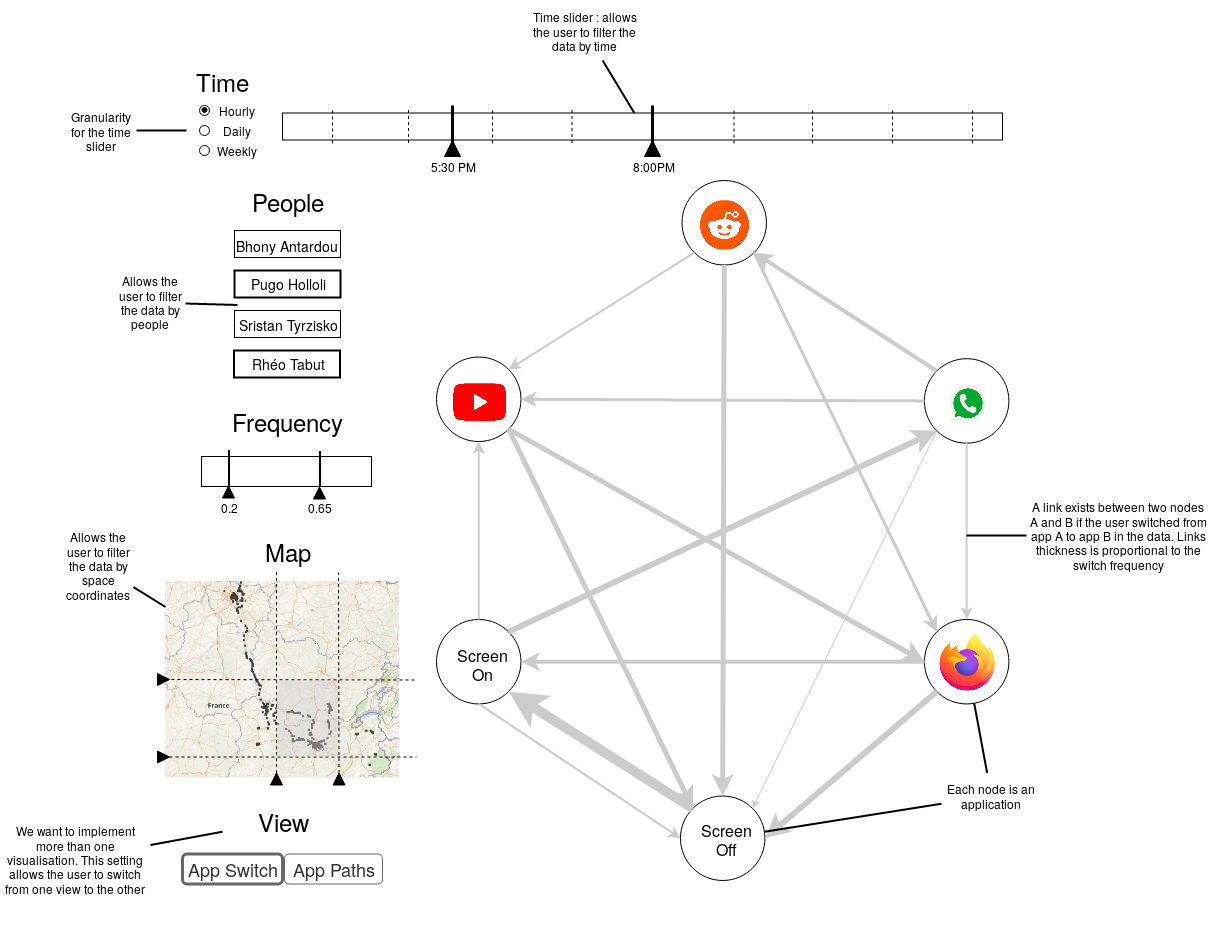
\includegraphics[height=300px]{sketches/AppGraph} \end{center}
		
		\subsection{Radial Tree}
		\begin{center} 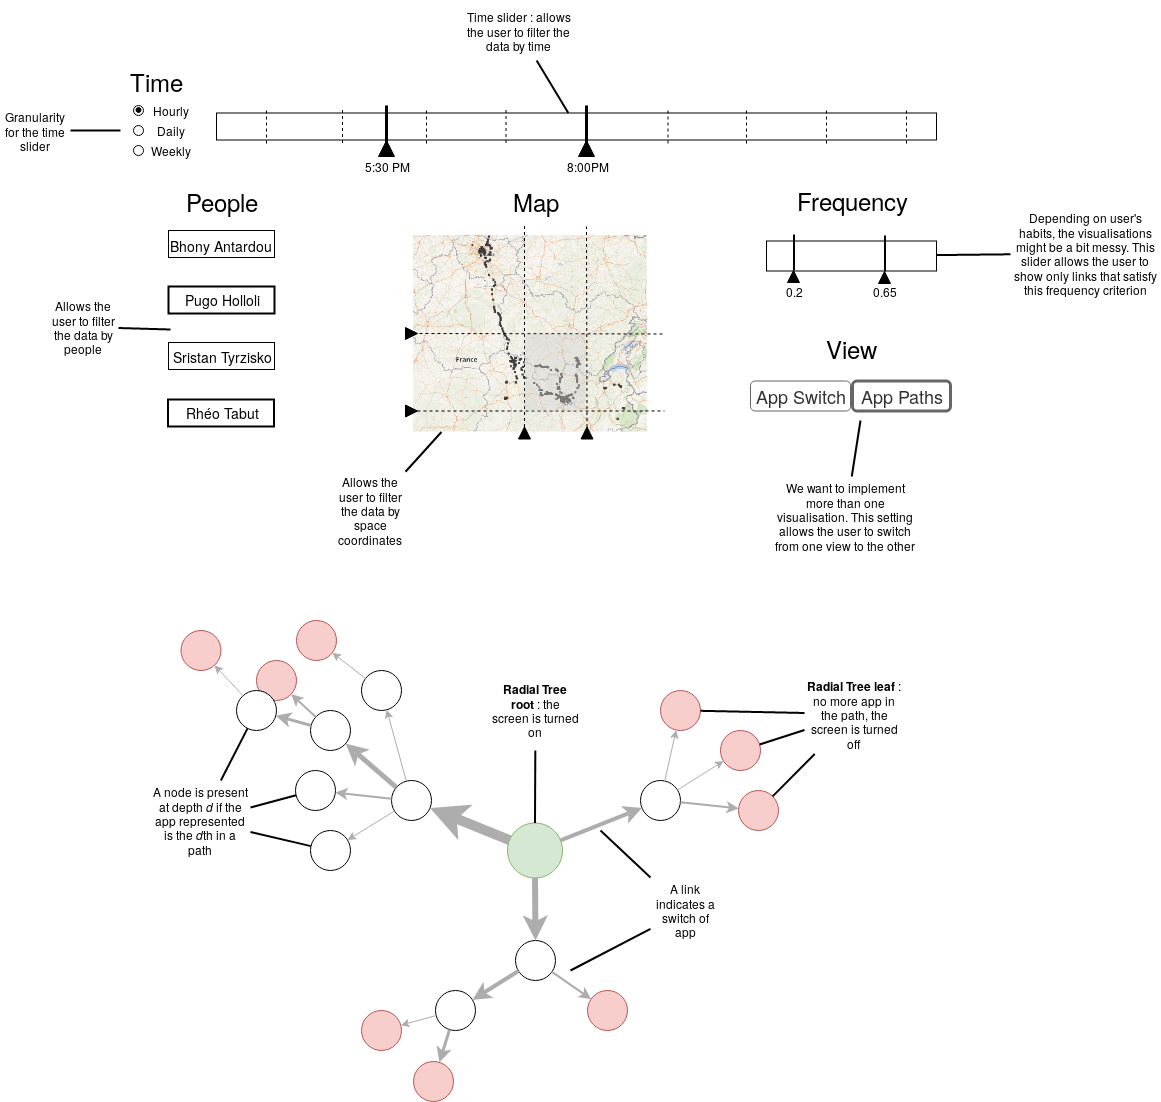
\includegraphics[height=300px]{sketches/AppRadTree} \end{center}
\end{document}